
\section{Global Camera Calibration}
\label{sec:global-calib}


To calibrate the multiple cameras, we follow the common framework consists of searching for feature point correspondences and minimizing reprojection errors. 
%
Because of the lack of the features in indoor scenes and the high requirement of the quality of the calibration, we use a $6\times7$ checkerboard with squares of 117 mm which can be made easily for the accuracy and robustness. 

%
An user holding the checkboard could move in front of the cameras freely in the working space. 
At each moment, the 8 cameras capture images simultaneously. 
%
The checkerboard is simultaneously seen in three or four views usually. 
%
Our system is flexible enough while it does not require that the checkboard must be visible under all points of view.
%
Then the 42 corners on the checkerboard can be detected in each local group.
%
For each time $t$, denote the group of cameras that can see the checkboard corners as $\mathcal{C}^t$. The 3D coordinates of the 42 corner points are denoted as $\{\vb{p}^{t}_{i}\}_{i=1,\ldots, 42}$, while their corresponding 2D coordinates detected in each image captured by the camera $c_j \in \mathcal{C}^{t}$ are $\{\vb{x}^{t}_{ji}\}$. 



While the user holding the checkboard moves around, we can capture $T$ groups of checkboard images and detect the corners at each time. 
%
To make the optimization result be more consistent to the whole system, we also use the images with checkerboard on the ground which allows the checkerboard corners can be seen in all the 8 cameras, as shown in Figure~\ref{fig:checkerboard}. This will help to reduce the accumulative error and inconsistence caused by the pairwise calibration. 
%Typically, our system could
\xj{Discussion on the range of T.}

According to the projection equation defined in Eq.~\ref{eq:cam-proj}, our calibration method optimizes the camera parameters to minimize the projection errors. Considering the $T$ groups of images together, the projection error is defined as: 
%
\begin{equation} \label{eq:global-proj-error}
E(\mathbf{M}_{j},\mathbf{p}^{t}_{i})=\sum_{t}\sum_{j\in \mathcal{C}^{t}}\sum_{i} \big( \hat{\vb{x}}(\vb{K}_{j},\mathbf{M}_{j}, \vb{p}^{t}_{i})-\mathbf{x}^{t}_{ji} \big)^{2},
\end{equation}
%
where $\hat{\vb{x}}(\vb{K}_{j},\mathbf{M}_{j}, \mathbf{p}_{i})$ is the estimated 2D positions of a 3D point $\vb{p}^{t}_{i}$ in the image plane of the camera $c_j$ with its parameters $\camin_j$ and $\camex_j$.


The above optimization could be solved by the Sparse Bundle Adjustment package~\cite{lour09}, which uses a Levenberg-Marquardt technique to optimize the parameters iteratively. 
Inevitably, this algorithm only finds a local optimal. 
A good initialization is required to get a good results. 


Though sequentially calibrate the neighboring cameras leads to accumulated errors, it could provide an initialization for the global optimization.
% 
We use the toolbox Kalibr~\cite{Maye2013Self} to obtain the intrinsic parameters and the initial extrinsic parameters of neighboring cameras sequentially. 
%
Then we estimate the 3D coordinates $\mathbf{p}^{t}_{ji}$ of each corner from the corresponding 2D coordinates by triangulation.
%where $n$ is the number of the views that the checkerboard can be seen in at the same time.
%
After the initial calibration, we globally optimize the extrinsic parameters and the 3D coordinates of each corner.

%\subsection{Multi-camera system}

\comments{
We employ 8 camera pods around the working space looking inwards for a full capture as shown in Figure~\ref{fig:rig}. Each camera pod consists of one color camera and two Near Infra-Red cameras. A laser pointer is used to produce special patterns.
From the two images of the projected patterns captured by the two NIR cameras, a depth map can be estimated using PatchMatch stereo algorithm~\cite{Bleyer2011PatchMatch}.
% it depth images can be achieved by the 2  using depth estimation methods.


%\subsection{Camera model}
Let $\mathbf{p}=(x,y,z,1)^{T}$ be the homogeneous coordinate of a point $P$ in the 3D space, and $\mathbf{x}=(u,v,1)^{T}$ the homogeneous coordinates of its projected point on an image plane, the perspective projection of a pin-hole camera is usually described as
\begin{equation}
z_{p}\mathbf{x}=\mathbf{K}\mathbf{M}\mathbf{p},
\end{equation}
where $z_{p}$ is the projective depth of point $P$, $\mathbf{K}$ and $\mathbf{M}$ are the intrinsic and extrinsic parameters of the camera.
}



%\subsection{Initial calibration}
The $\mathbf{K}$ and initial $\mathbf{M}$ of each camera are calibrated by Kalibr~\cite{Maye2013Self} pairwisely because of the lack of the common overlapping fields of view, including the 8 color cameras' extrinsic parameters $\{\mathbf{M}_{i}\}_{i=1,\ldots,8}$. The extrinsic parameters from the 2 NIR cameras to the color camera in the same camera pod are also achieved, but these extrinsic parameters are fixed and used to estimate the depth in each view.

%\subsection{Global optimization}




\begin{figure}[ht]
%
\begin{minipage}[b]{.48\linewidth}
  \centering
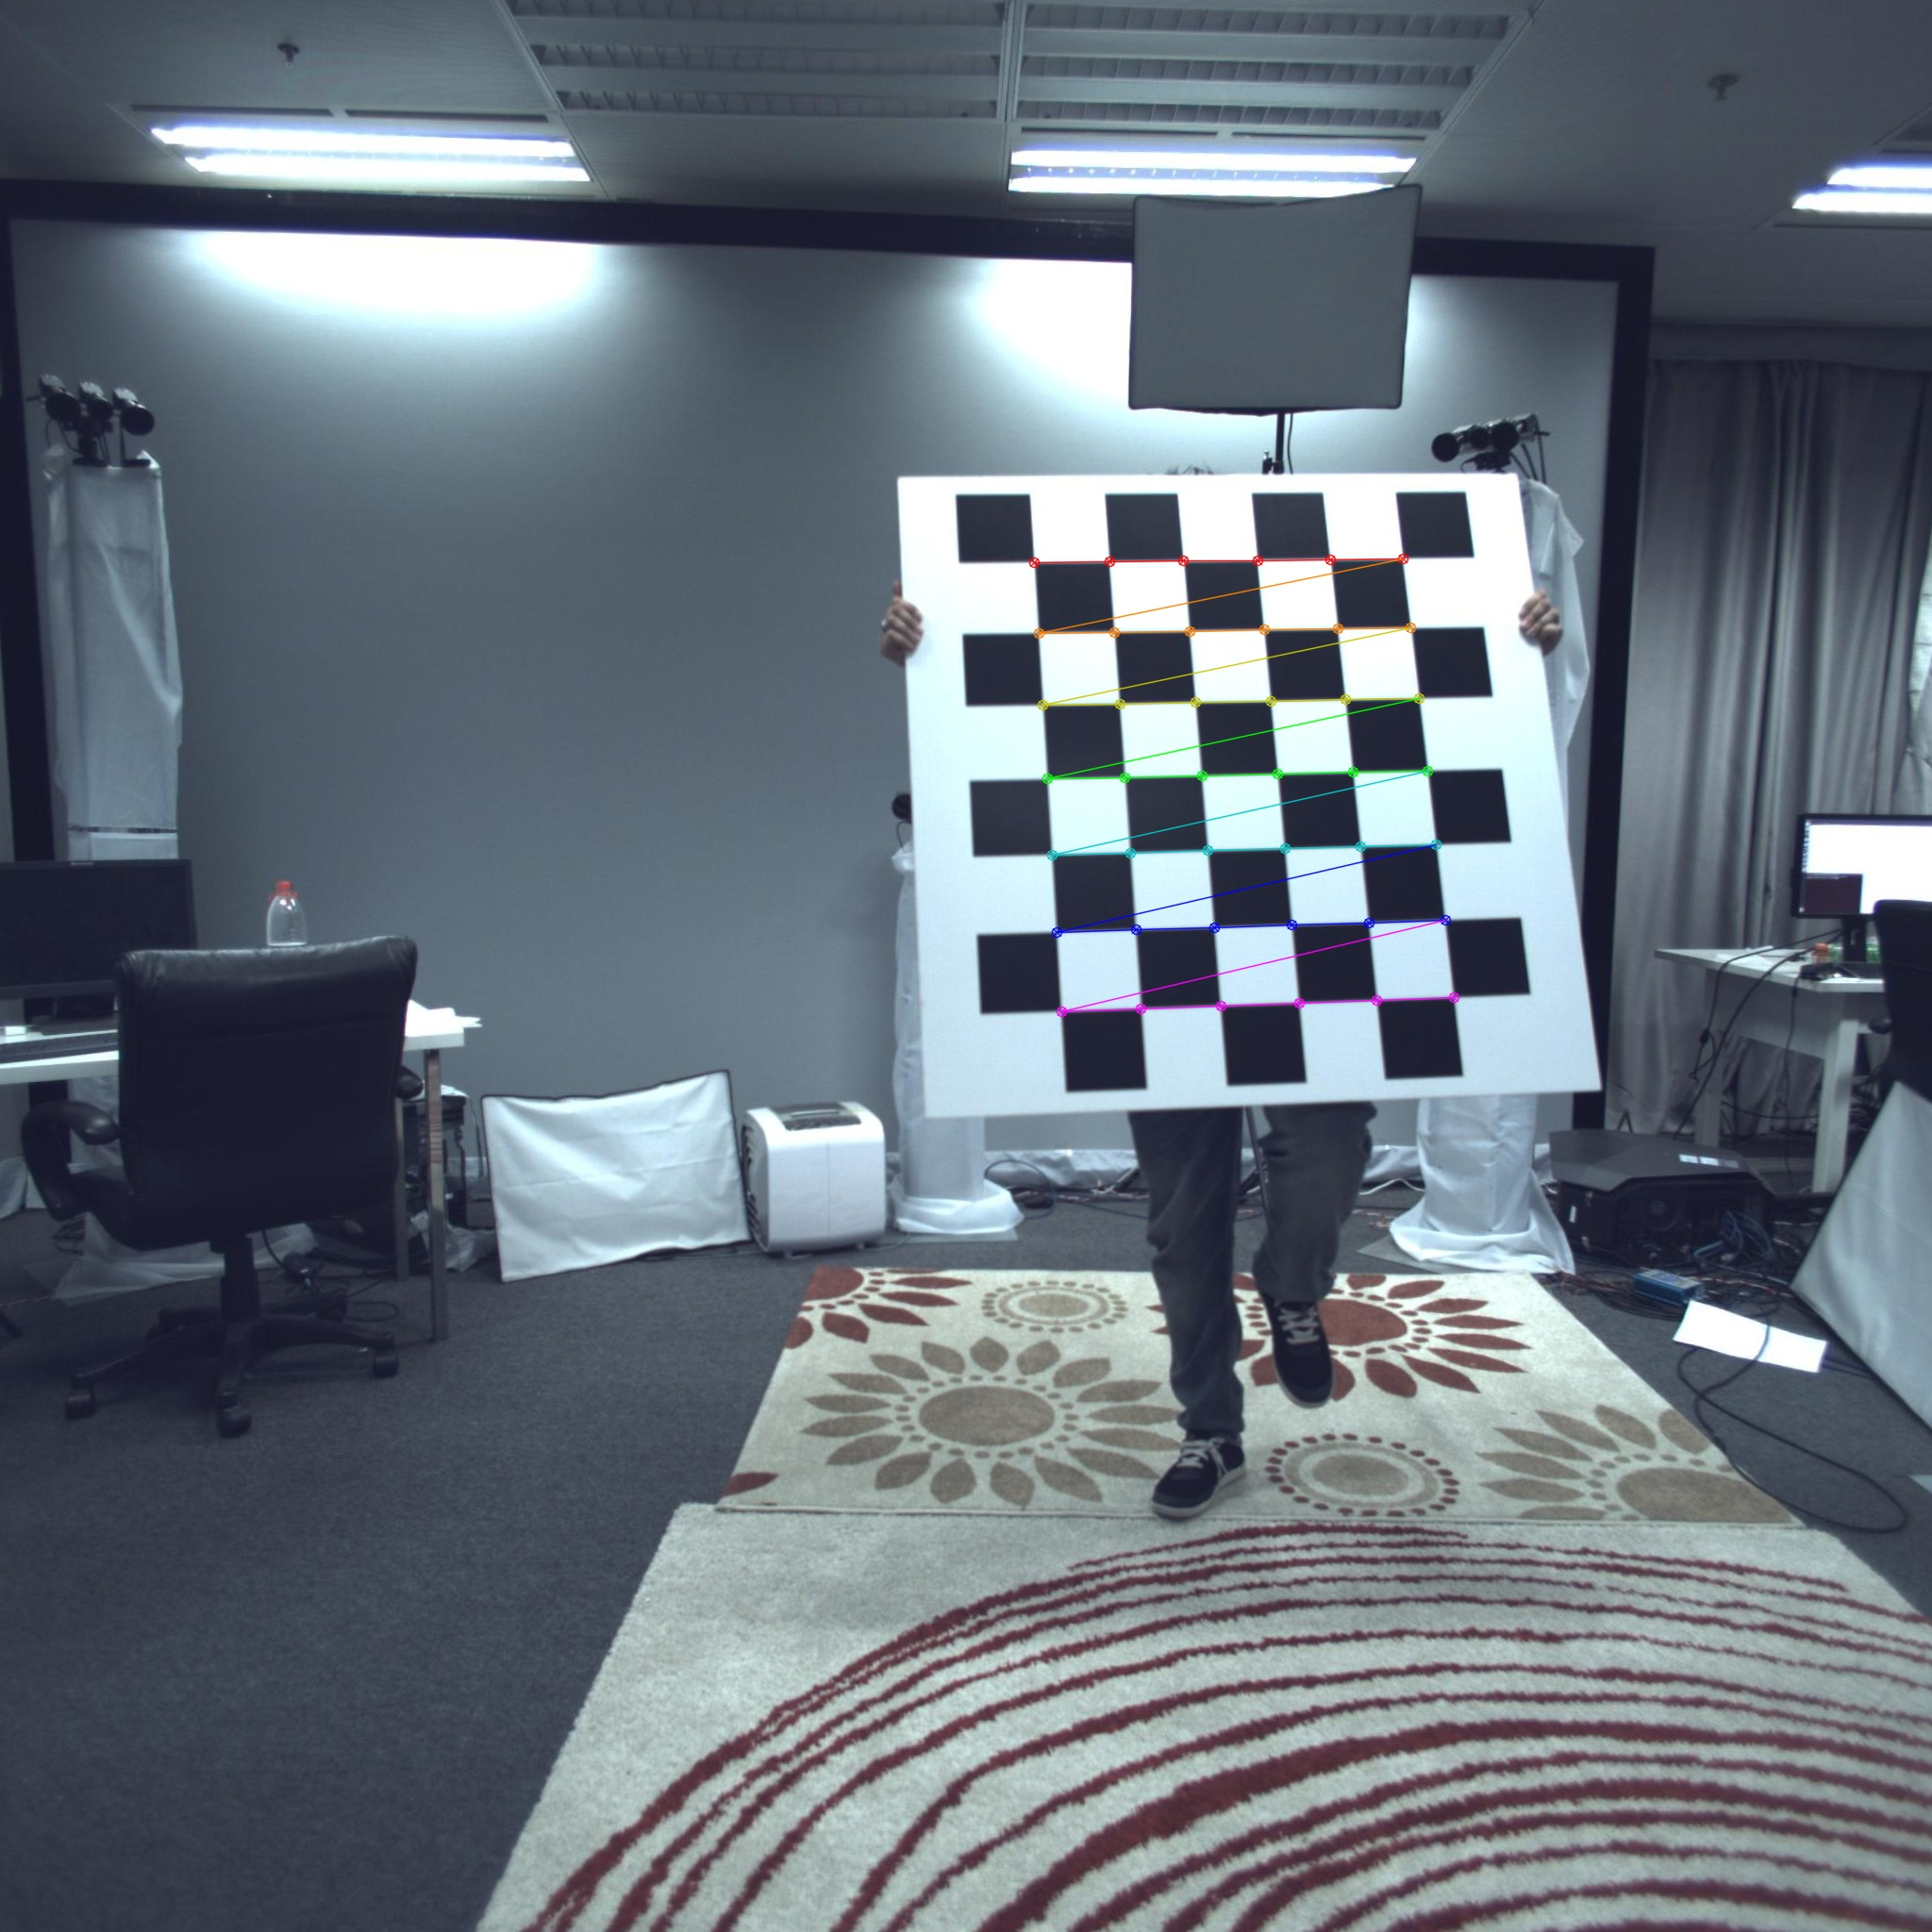
\includegraphics[scale=0.058]{image/free.jpg}
  \vspace{0cm}
  \centerline{(a)}\medskip
\end{minipage}
\hfill
\begin{minipage}[b]{0.48\linewidth}
  \centering
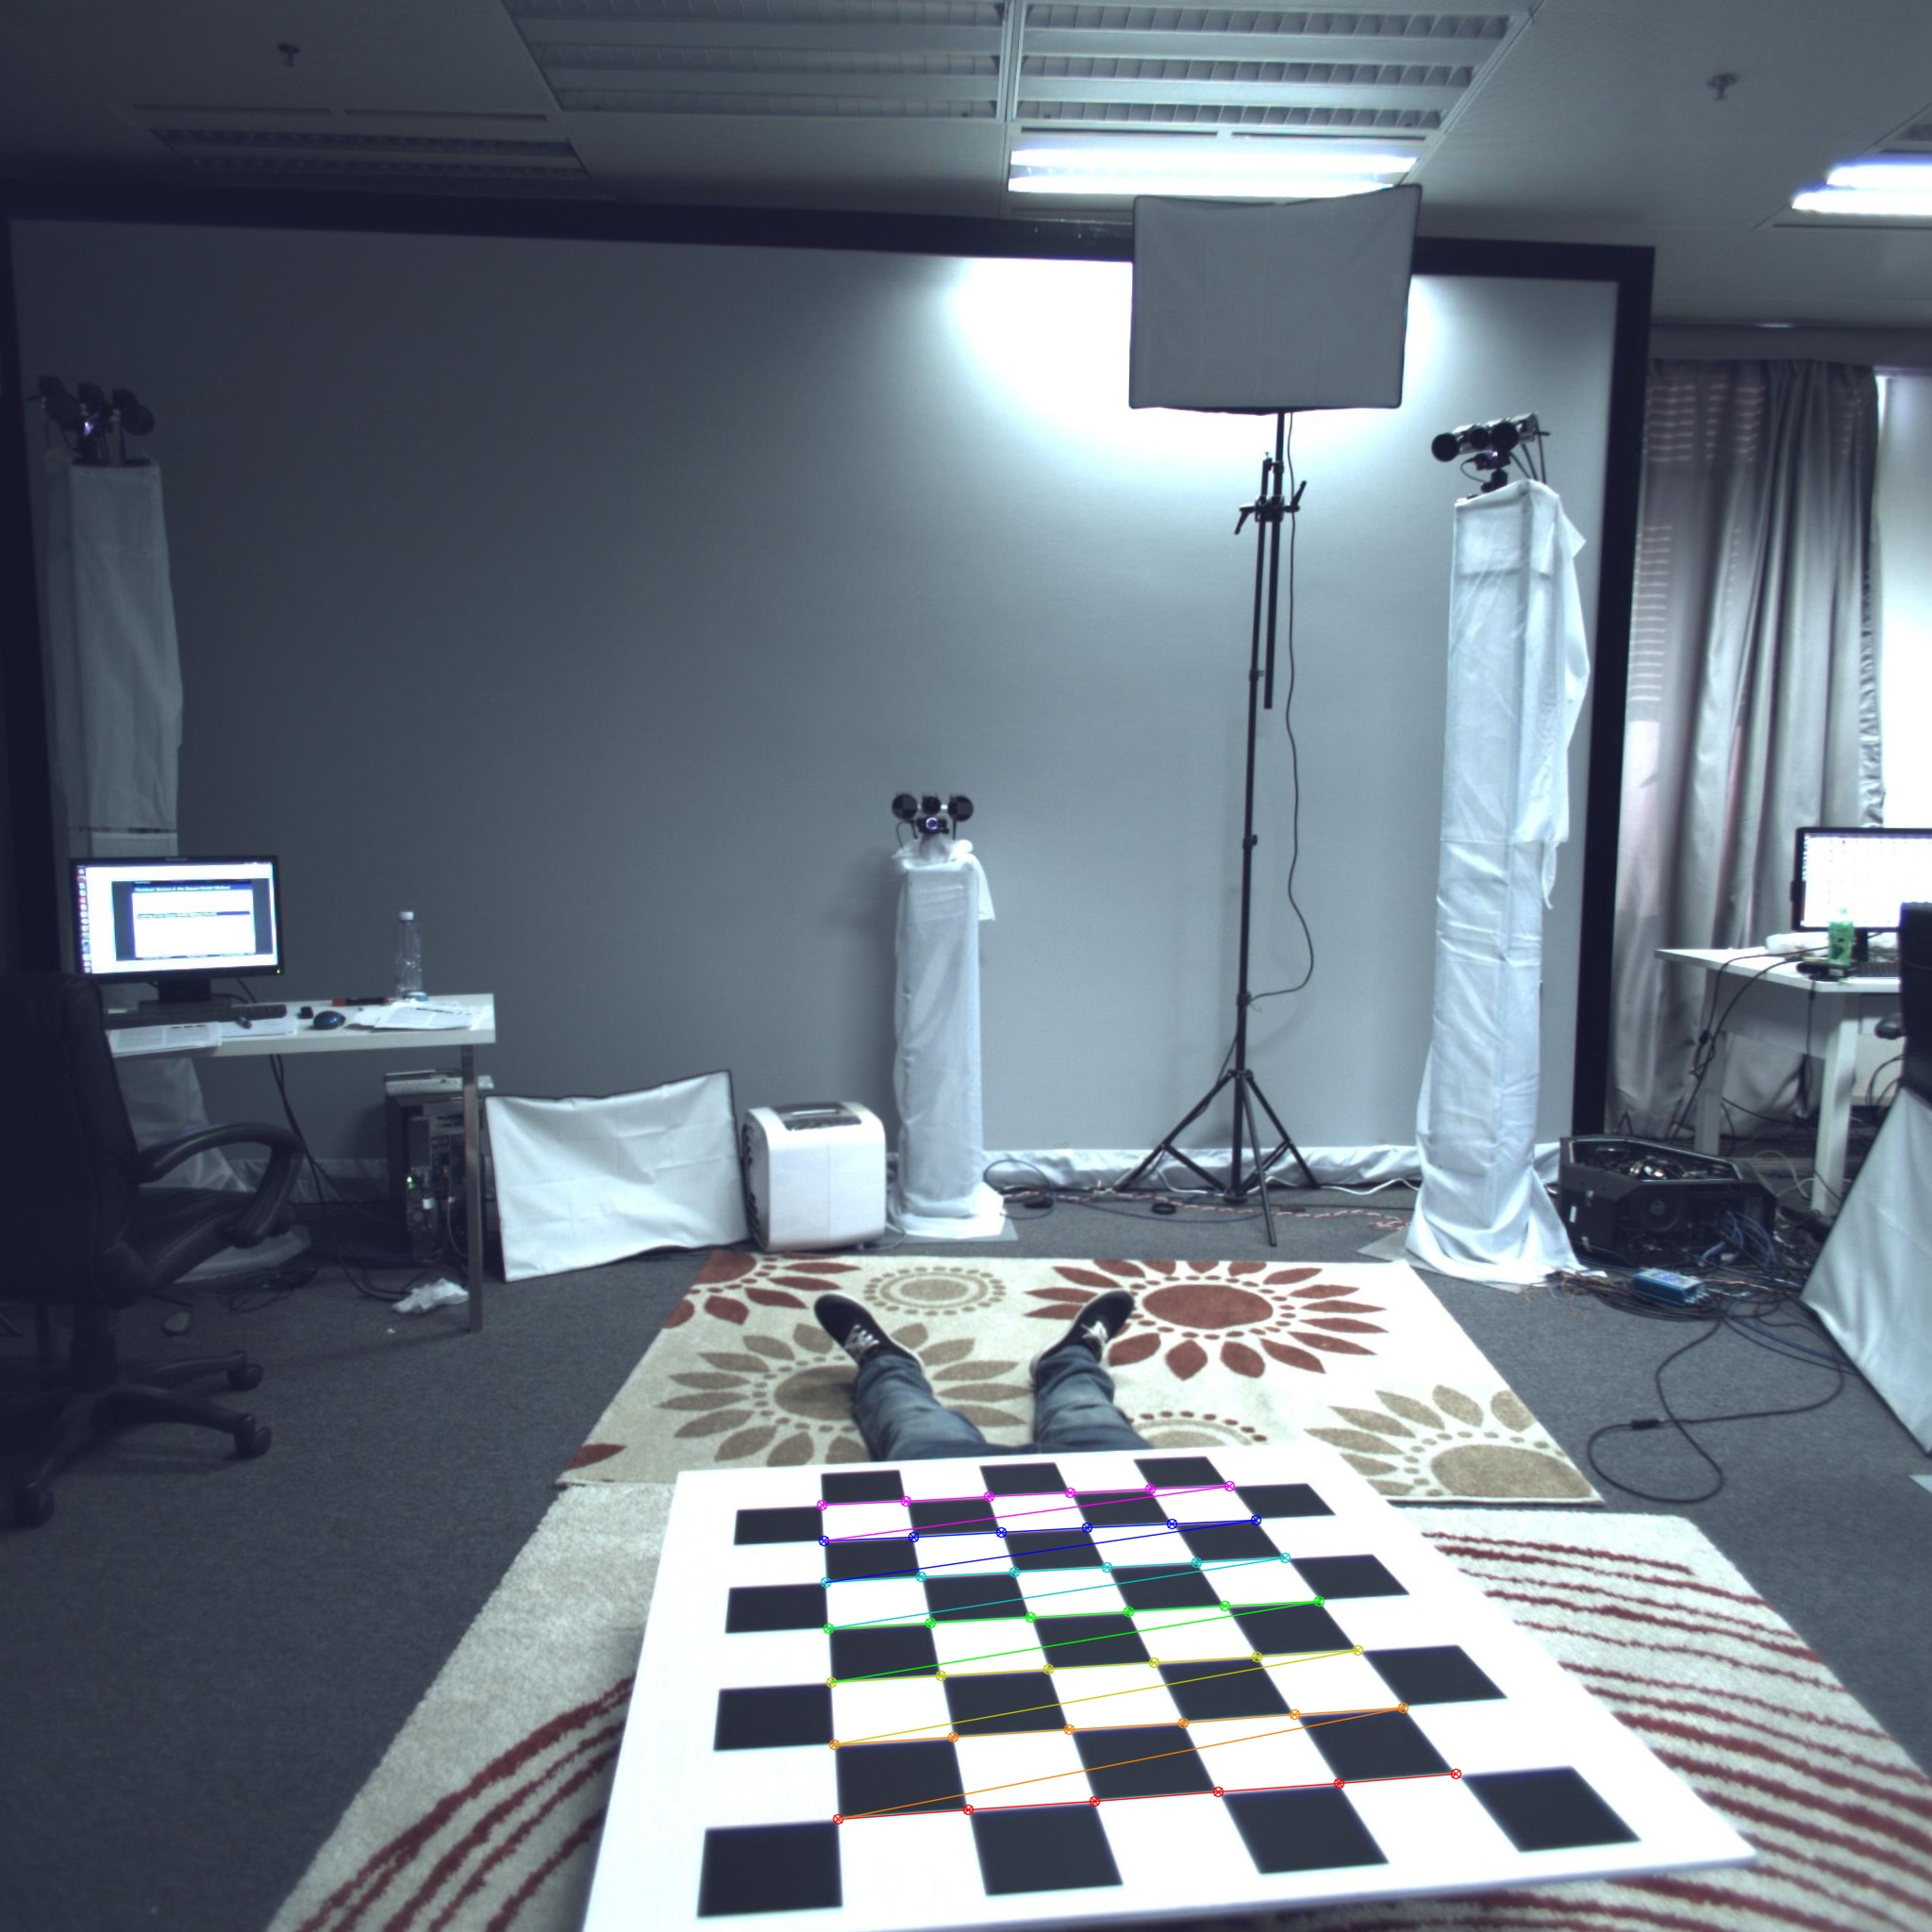
\includegraphics[scale=0.058]{image/ground.jpg}
  \vspace{0cm}
  \centerline{(b)}\medskip
\end{minipage}
%
\caption{Results of the checkerboard corners detection. (a): Results when the user moves freely. (b): Results when the checkerboard is on the ground. }
\label{fig:checkerboard}
\end{figure}



\section{point cloud registration}
\label{sec:registration}

We achieve the depth data from the 2 NIR cameras using depth estimation methods~\cite{Bleyer2011PatchMatch}. Although after the global optimization, we can get a result with less reprojection error, but it may not be the optimal solution to the 3D reconstruction because the quality of depth estimation also influence the final result. If the depth and camera parameters are both accurate enough, the point clouds of different views should align very well.
\md{However, the depth estimation methods based on NIR cameras are not suitable for all cases and are not robust enough especially for light-absorbing material like black hair. Moreover, the depth estimation may be affected by many factors like the quality of the laser pointer, the interaction effect on the camera pods which are arranged towards each other caused by the laser and similarity. Although there have been many research on it, the error cannot be avoided completely.}
%However, the error cannot be avoided completely.
\xj{what error? caused by what?}

We reconstruct the point cloud of one view using the rgb and depth data, found the distortion on the boundary of the model, especially near the head, as shown in Figure~\ref{fig:deptherror}. Moreover, although the reprojection error after the global optimization mentioned in the last section is at sub-pixel level, which can prove the high accuracy of our calibration result, we still find the separation between the point cloud of different views when we map the depth to the entire model, effecting the quality of reconstruction. These deficiencies are mainly caused by the depth estimation.
%
To minimize the error from depth data and achieve high-quality reconstruction results, we use ICP to map the inaccurate depth to a 3D model by point cloud registration.

\begin{figure*}[ht]
  \centering
\subfigure[]{
\begin{minipage}[c]{.22\linewidth}
\centering
  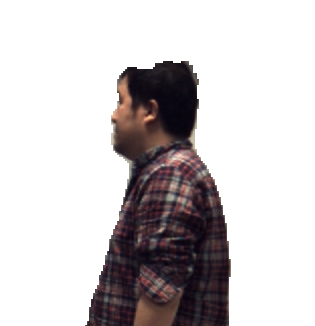
\includegraphics[width=4cm]{image/depth_error_rgb.png}
\end{minipage}
}%
\subfigure[]{
\begin{minipage}[c]{.22\linewidth}
\centering
  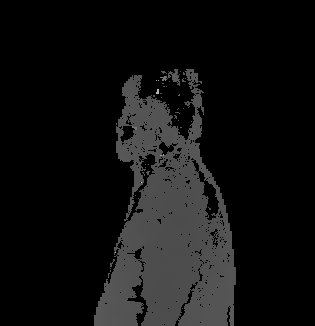
\includegraphics[width=4cm]{image/depth_error_depth.png}
\end{minipage}
}
\subfigure[]{
\begin{minipage}[c]{.22\linewidth}
\centering
  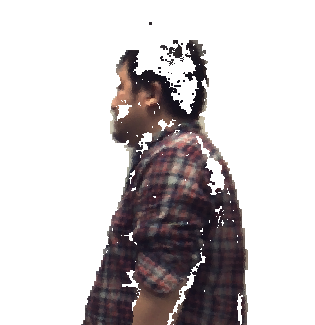
\includegraphics[width=4cm]{image/depth_error_pc.png}
\end{minipage}
}
\subfigure[]{
\begin{minipage}[c]{.22\linewidth}
\centering
  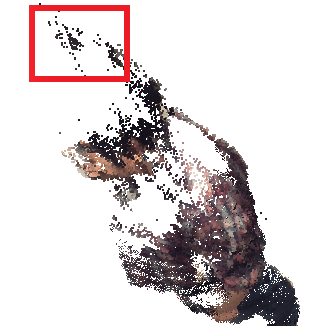
\includegraphics[width=4cm]{image/depth_error_pc_2.png}
\end{minipage}
}
\caption{(a): RGB data. (b): Depth data. (c): The point cloud reconstruted by (a) and (b). (d): (c) in another view. The distortion near the head of the model of a single view which is caused by the inaccurate depth estimation can seen in the red box.}
\label{fig:deptherror}
\end{figure*}


For each point reconstructed by the depth image, we consider an estimation
\begin{equation}
\mathbf{\tilde{P}}_{ij}=f_{i}(\mathbf{P}_{j}),
\end{equation}
where $\mathbf{P}_{j}$ is the true 3D coordinates in the camera coordinate system. $f_{i}$ is a nonlinear function for view $i$, represent the depth influence. $\mathbf{\tilde{P}}_{ij}$ is the 3D coordinates we get from the depth data and intrinsic parameters in view $i$. With the extrinsic parameter, we can transform all the points into the world coordinate system. The estimation can be written as
\begin{equation}
\mathbf{\hat{P}}_{gj}=g(\mathbf{K_{ex}}_{i})f_{i}(\mathbf{P}_{j}),
\end{equation}
where $\mathbf{\hat{P}}_{gj}$ is the 3D coordinates in the world coordinate system we reconstruct from the depth and camera parameters. ICP can be replaced as a rigid transform to all views
\begin{equation}
\mathbf{\tilde{\hat{P}}}_{gj}=M_{i}g(\mathbf{K_{ex}}_{i})f_{i}(\mathbf{P}_{j})=g(\mathbf{K_{ex}}_{i})M_{i}f_{i}(\mathbf{P}_{j}),
\end{equation}
where $\mathbf{\tilde{\hat{P}}}_{gj}$ is the coordinates of the point after the alignment. The transform $M_{i}$ can refine the error caused by $f_{i}$, and improve the quality of the result of 3D reconstruction.

We choose the point cloud of view 1 as the reference, align the point cloud of view 2 to it, combine the result of the two views, then align the point cloud of view 3 to the combined result and so on. Each ICP process produce a transformation matrix, then we can map the inaccurate depth to a high-quality 3D model using the rigid transformation.


\xj{Show depth maps from 8 views. Show three fused models from pairwisely estimated camera parameters, globally estimated camera parameters, and after icp registration.  }
\md{(I am finding a better way to show the depth map. I don't know whether there is any mature software to show depth map. Or i will write a program to show it.)}

% References should be produced using the bibtex program from suitable
% BiBTeX files (here: strings, refs, manuals). The IEEEbib.bst bibliography
% style file from IEEE produces unsorted bibliography list.
% -------------------------------------------------------------------------

